\documentclass[14pt]{extbook}
\usepackage{multicol, enumerate, enumitem, hyperref, color, soul, setspace, parskip, fancyhdr} %General Packages
\usepackage{amssymb, amsthm, amsmath, latexsym, units, mathtools} %Math Packages
\everymath{\displaystyle} %All math in Display Style
% Packages with additional options
\usepackage[headsep=0.5cm,headheight=12pt, left=1 in,right= 1 in,top= 1 in,bottom= 1 in]{geometry}
\usepackage[usenames,dvipsnames]{xcolor}
\usepackage{dashrule}  % Package to use the command below to create lines between items
\newcommand{\litem}[1]{\item#1\hspace*{-1cm}\rule{\textwidth}{0.4pt}}
\pagestyle{fancy}
\lhead{Progress Quiz 7}
\chead{}
\rhead{Version A}
\lfoot{3510-5252}
\cfoot{}
\rfoot{Summer C 2021}
\begin{document}

\begin{enumerate}
\litem{
Write the equation of the graph presented below in the form $f(x)=ax^2+bx+c$, assuming  $a=1$ or $a=-1$. Then, choose the intervals that $a, b,$ and $c$ belong to.
\begin{center}
    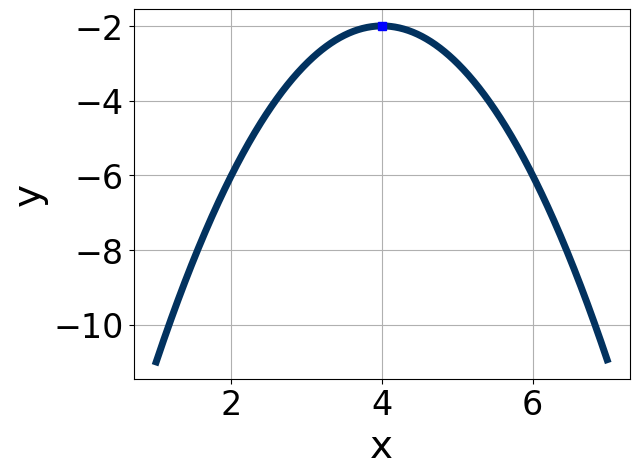
\includegraphics[width=0.5\textwidth]{../Figures/quadraticGraphToEquationA.png}
\end{center}
\begin{enumerate}[label=\Alph*.]
\item \( a \in [-1.3, 0], \hspace*{5mm} b \in [4, 10], \text{ and } \hspace*{5mm} c \in [-18, -16] \)
\item \( a \in [0.4, 1.5], \hspace*{5mm} b \in [4, 10], \text{ and } \hspace*{5mm} c \in [10, 15] \)
\item \( a \in [0.4, 1.5], \hspace*{5mm} b \in [-10, -5], \text{ and } \hspace*{5mm} c \in [10, 15] \)
\item \( a \in [-1.3, 0], \hspace*{5mm} b \in [-10, -5], \text{ and } \hspace*{5mm} c \in [-18, -16] \)
\item \( a \in [-1.3, 0], \hspace*{5mm} b \in [-10, -5], \text{ and } \hspace*{5mm} c \in [-14, -9] \)

\end{enumerate} }
\litem{
Solve the quadratic equation below. Then, choose the intervals that the solutions $x_1$ and $x_2$ belong to, with $x_1 \leq x_2$.\[ 25x^{2} -60 x + 36 = 0 \]\begin{enumerate}[label=\Alph*.]
\item \( x_1 \in [-0.17, 0.3] \text{ and } x_2 \in [5.29, 6.08] \)
\item \( x_1 \in [0.41, 0.76] \text{ and } x_2 \in [2.12, 2.75] \)
\item \( x_1 \in [0.34, 0.44] \text{ and } x_2 \in [2.63, 4.78] \)
\item \( x_1 \in [1.11, 1.3] \text{ and } x_2 \in [0.47, 1.4] \)
\item \( x_1 \in [29.67, 30.12] \text{ and } x_2 \in [29.21, 30.44] \)

\end{enumerate} }
\litem{
Factor the quadratic below. Then, choose the intervals that contain the constants in the form $(ax+b)(cx+d); b \leq d.$\[ 24x^{2} +2 x -15 \]\begin{enumerate}[label=\Alph*.]
\item \( a \in [10.31, 12.79], \hspace*{5mm} b \in [-3, 0], \hspace*{5mm} c \in [1.45, 3.07], \text{ and } \hspace*{5mm} d \in [0, 7] \)
\item \( a \in [1.21, 2.53], \hspace*{5mm} b \in [-3, 0], \hspace*{5mm} c \in [11.98, 12.04], \text{ and } \hspace*{5mm} d \in [0, 7] \)
\item \( a \in [0.14, 1.79], \hspace*{5mm} b \in [-20, -12], \hspace*{5mm} c \in [-0.18, 1.72], \text{ and } \hspace*{5mm} d \in [18, 22] \)
\item \( a \in [2.38, 4.11], \hspace*{5mm} b \in [-3, 0], \hspace*{5mm} c \in [4.37, 6.28], \text{ and } \hspace*{5mm} d \in [0, 7] \)
\item \( \text{None of the above.} \)

\end{enumerate} }
\litem{
Write the equation of the graph presented below in the form $f(x)=ax^2+bx+c$, assuming  $a=1$ or $a=-1$. Then, choose the intervals that $a, b,$ and $c$ belong to.
\begin{center}
    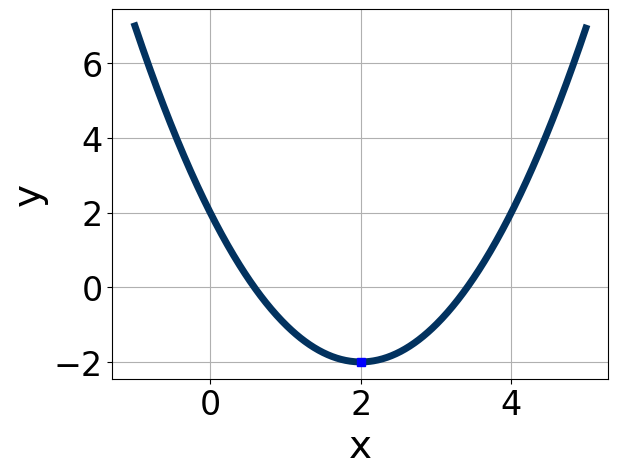
\includegraphics[width=0.5\textwidth]{../Figures/quadraticGraphToEquationCopyA.png}
\end{center}
\begin{enumerate}[label=\Alph*.]
\item \( a \in [1, 3], \hspace*{5mm} b \in [-6, -3], \text{ and } \hspace*{5mm} c \in [1, 4] \)
\item \( a \in [-2, 0], \hspace*{5mm} b \in [-6, -3], \text{ and } \hspace*{5mm} c \in [-7, -4] \)
\item \( a \in [-2, 0], \hspace*{5mm} b \in [3, 7], \text{ and } \hspace*{5mm} c \in [-7, -4] \)
\item \( a \in [1, 3], \hspace*{5mm} b \in [3, 7], \text{ and } \hspace*{5mm} c \in [1, 4] \)
\item \( a \in [1, 3], \hspace*{5mm} b \in [3, 7], \text{ and } \hspace*{5mm} c \in [6, 8] \)

\end{enumerate} }
\litem{
Graph the equation below.\[ f(x) = (x-1)^2 - 15 \]\begin{enumerate}[label=\Alph*.]
\begin{multicols}{2}\item 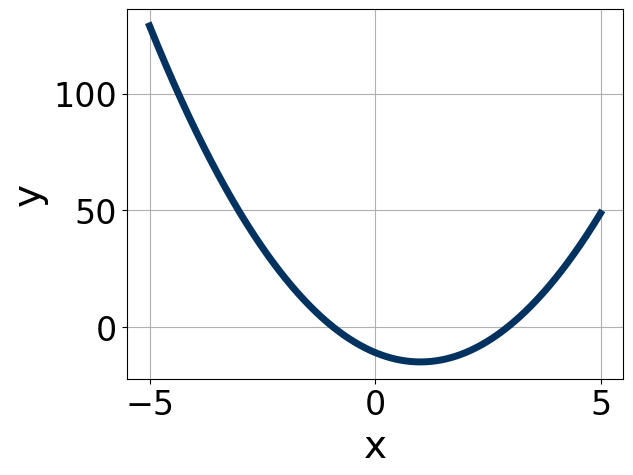
\includegraphics[width = 0.3\textwidth]{../Figures/quadraticEquationToGraphAA.png}\item 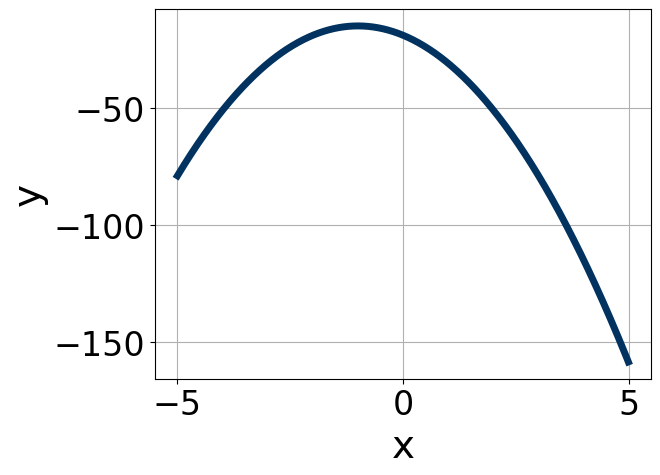
\includegraphics[width = 0.3\textwidth]{../Figures/quadraticEquationToGraphBA.png}\item 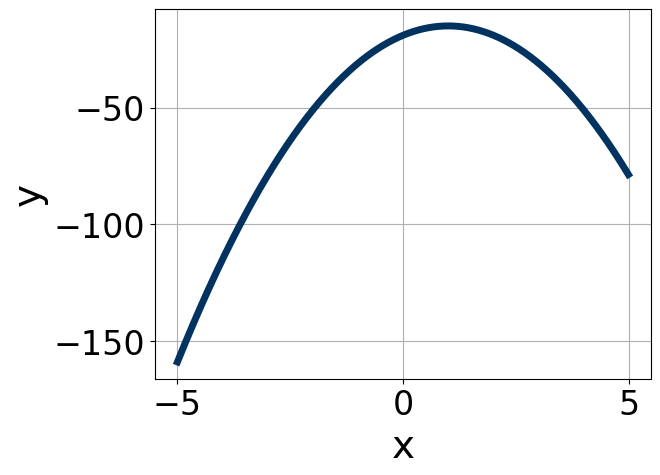
\includegraphics[width = 0.3\textwidth]{../Figures/quadraticEquationToGraphCA.png}\item 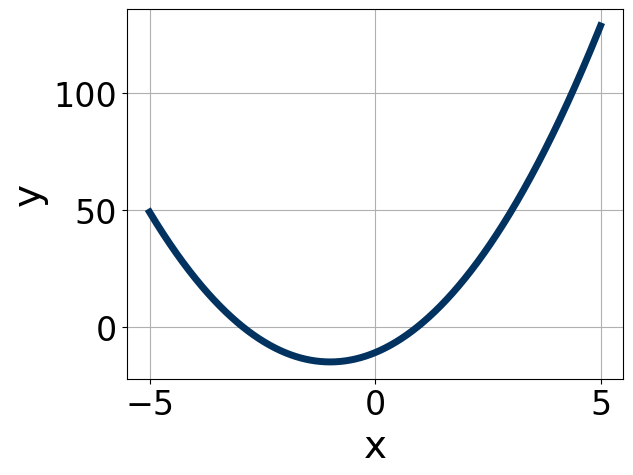
\includegraphics[width = 0.3\textwidth]{../Figures/quadraticEquationToGraphDA.png}\end{multicols}\item None of the above.
\end{enumerate} }
\litem{
Solve the quadratic equation below. Then, choose the intervals that the solutions belong to, with $x_1 \leq x_2$ (if they exist).\[ -19x^{2} -13 x + 4 = 0 \]\begin{enumerate}[label=\Alph*.]
\item \( x_1 \in [-2.01, -0.76] \text{ and } x_2 \in [-0.3, 0.68] \)
\item \( x_1 \in [-23.26, -21.68] \text{ and } x_2 \in [21.39, 22.14] \)
\item \( x_1 \in [-0.7, 0.91] \text{ and } x_2 \in [0.37, 1.52] \)
\item \( x_1 \in [-5.5, -3.85] \text{ and } x_2 \in [17.2, 17.52] \)
\item \( \text{There are no Real solutions.} \)

\end{enumerate} }
\litem{
Solve the quadratic equation below. Then, choose the intervals that the solutions $x_1$ and $x_2$ belong to, with $x_1 \leq x_2$.\[ 12x^{2} -11 x -36 = 0 \]\begin{enumerate}[label=\Alph*.]
\item \( x_1 \in [-16.44, -15.72] \text{ and } x_2 \in [26.49, 27.56] \)
\item \( x_1 \in [-3.53, -2.27] \text{ and } x_2 \in [1.11, 1.35] \)
\item \( x_1 \in [-1.36, -0.79] \text{ and } x_2 \in [1.98, 2.27] \)
\item \( x_1 \in [-0.82, 0.13] \text{ and } x_2 \in [6.53, 7] \)
\item \( x_1 \in [-4.47, -3.68] \text{ and } x_2 \in [0.71, 0.81] \)

\end{enumerate} }
\litem{
Graph the equation below.\[ f(x) = -(x-3)^2 - 19 \]\begin{enumerate}[label=\Alph*.]
\begin{multicols}{2}\item 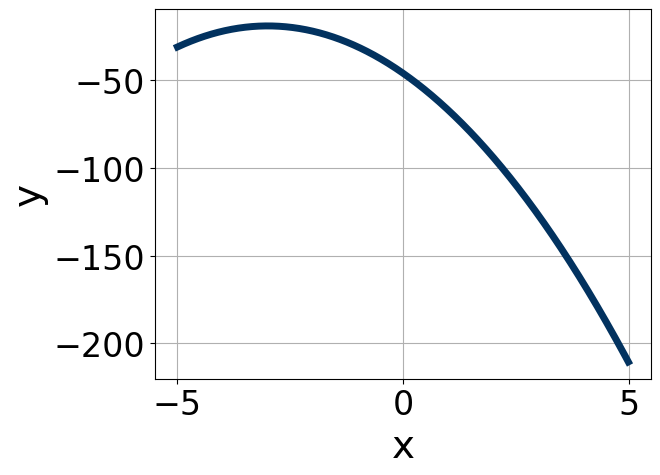
\includegraphics[width = 0.3\textwidth]{../Figures/quadraticEquationToGraphCopyAA.png}\item 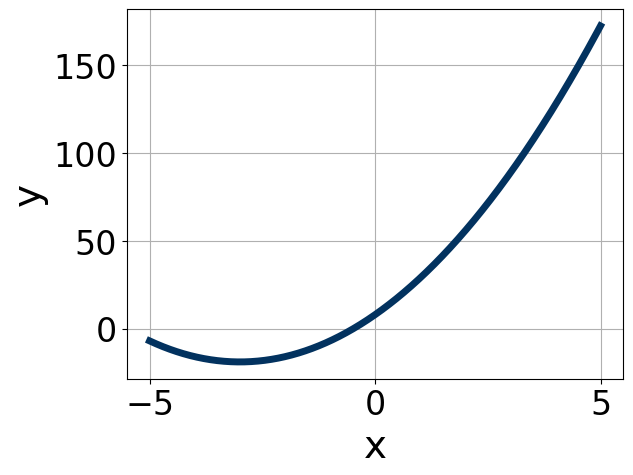
\includegraphics[width = 0.3\textwidth]{../Figures/quadraticEquationToGraphCopyBA.png}\item 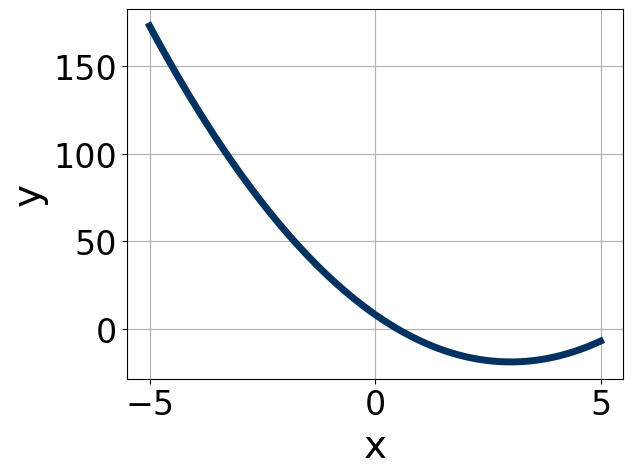
\includegraphics[width = 0.3\textwidth]{../Figures/quadraticEquationToGraphCopyCA.png}\item 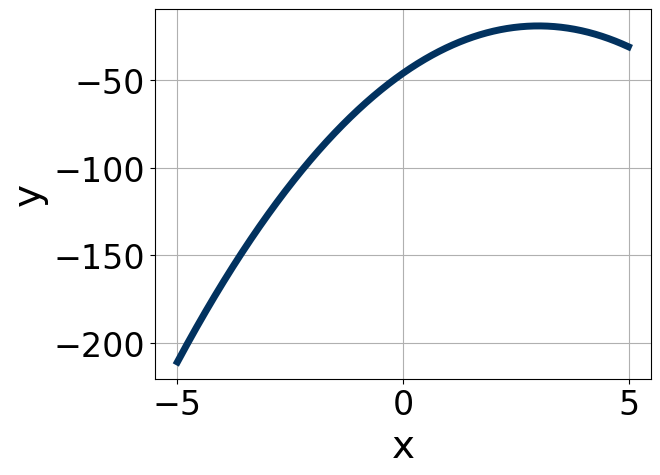
\includegraphics[width = 0.3\textwidth]{../Figures/quadraticEquationToGraphCopyDA.png}\end{multicols}\item None of the above.
\end{enumerate} }
\litem{
Solve the quadratic equation below. Then, choose the intervals that the solutions belong to, with $x_1 \leq x_2$ (if they exist).\[ 12x^{2} +7 x -9 = 0 \]\begin{enumerate}[label=\Alph*.]
\item \( x_1 \in [-1.2, -0.18] \text{ and } x_2 \in [0.9, 2.8] \)
\item \( x_1 \in [-2.69, -1.12] \text{ and } x_2 \in [-0.1, 1.2] \)
\item \( x_1 \in [-22.99, -21.32] \text{ and } x_2 \in [21, 23.8] \)
\item \( x_1 \in [-14.62, -14.4] \text{ and } x_2 \in [5.7, 8.9] \)
\item \( \text{There are no Real solutions.} \)

\end{enumerate} }
\litem{
Factor the quadratic below. Then, choose the intervals that contain the constants in the form $(ax+b)(cx+d); b \leq d.$\[ 24x^{2} +2 x -15 \]\begin{enumerate}[label=\Alph*.]
\item \( a \in [-0.18, 1.9], \hspace*{5mm} b \in [-24, -17], \hspace*{5mm} c \in [-0.9, 1.2], \text{ and } \hspace*{5mm} d \in [19, 23] \)
\item \( a \in [11.49, 13.43], \hspace*{5mm} b \in [-6, -1], \hspace*{5mm} c \in [1.4, 2.5], \text{ and } \hspace*{5mm} d \in [2, 11] \)
\item \( a \in [1.58, 2.63], \hspace*{5mm} b \in [-6, -1], \hspace*{5mm} c \in [10.2, 13.3], \text{ and } \hspace*{5mm} d \in [2, 11] \)
\item \( a \in [3.9, 5.36], \hspace*{5mm} b \in [-6, -1], \hspace*{5mm} c \in [4.6, 6.6], \text{ and } \hspace*{5mm} d \in [2, 11] \)
\item \( \text{None of the above.} \)

\end{enumerate} }
\end{enumerate}

\end{document}